\chapter{Analisis}
\label{chap:analysis}

\section{Analisis Aplikasi Sejenis}
\label{sec:analysis-similarapps}

Untuk pembuatan perangkat lunak dalam skripsi ini, ada empat buah perkakas \cl yang akan diamati sebagai aplikasi sejenis. Dua dari empat aplikasi pertama adalah \chromewebstorecli dan \textit{iTunes Search API}. Selain dua perkakas tersebut, ada dua perkakas lainnya yang bisa digunakan sebagai referensi, tetapi tidak dapat dieksplorasi, karena kedua aplikasi tersebut tidak berhasil dijalankan dengan sempurna, yaitu \ubercli dan \googlemapscli

\subsection{\chromewebstorecli\footnote{\href{https://github.com/pandawing/node-chrome-web-store-item-property-cli}{https://github.com/pandawing/node-chrome-web-store-item-property-cli}}}
\label{sec:similarapps-chromewebstore}

Perkakas \cl ini merupakan ekstensi dari sebuah aplikasi lain yang memiliki fungsi yang sama, yaitu Chrome \textit{Web Store Item Property}.\footnote{\href{https://github.com/pandawing/node-chrome-web-store-item-property}{https://github.com/pandawing/node-chrome-web-store-item-property}} Perangkat lunak \chromewebstorecli ini merupakan perangkat lunak yang akan memanggil fungsi API untuk mendapatkan metadata dari sebuah ekstensi pada \textit{web store} peramban Google Chrome. Perbedaan dari perkakas ini dengan aplikasi dasarnya adalah bahwa perkakas ini dapat digunakan sebagai perkakas \textit{command line}, sedangkan aplikasi dasarnya hanya bisa digunakan dalam perangkat lunak lainnya sebagai pemanggil fungsi API.

\subsubsection{Penggunaan}
\label{sec:similarapps-chromewebstore-usage}

Perkakas ini dapat digunakan melalui \textit{command prompt} dengan cara mengetikkan perintah sebagai berikut.

\begin{verbatim}
                     chrome-web-store-item-property <identifier>
\end{verbatim}

Dengan \verb|identifier| berupa ID dari ekstensi yang diinginkan. Jadi, misalkan pengguna memasukkan \verb|gighmmpiobklfepjocnamgkkbiglidom| sebagai ID yang akan digunakan sebagai \textit{identifier}, maka perkakas ini akan mengembalikan metadata dari ekstensi ``AdBlock'' sebagai keluarannya. Contoh penggunaan perkakas ini dapat dilihat di gambar \ref{fig:similarapps-chromewebstorecli}.

\begin{figure}[ht]
    \centering
    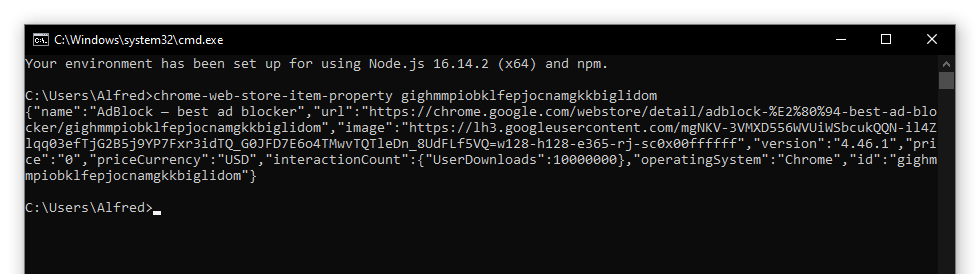
\includegraphics[width=0.75\linewidth]{chromewebstorecli}
    \caption[Contoh penggunaan perkakas \chromewebstorecli]{Contoh penggunaan perkakas \chromewebstorecli.}
    \label{fig:similarapps-chromewebstorecli}
\end{figure}

Sedangkan, keluaran dari perkakas ini merupakan sebuah objek JSON dengan properti-properti sebagai berikut.

\begin{itemize}
	\item \verb|name|\\
	Nama dari ekstensi yang dicari metadatanya.
	\item \verb|url|\\
	URL halaman web dari ekstensi yang dicari di \textit{web store} Google Chrome.
	\item \verb|image|\\
	Logo (dan ikon \textit{thumbnail}) dari ekstensi yang dicari metadatanya.
	\item \verb|version|\\
	Nomor versi dari ekstensi.
	\item \verb|price|\\
	Harga dari ekstensi. Jika ekstensi tidak memiliki harga yang perlu dibayarkan (gratis), properti ini akan bernilai \verb|0|.
	\item \verb|priceCurrency|\\
	Kode mata uang dari harga ekstensi. Jika ekstensi tidak memiliki harga yang perlu dibayarkan, properti ini akan berisi ``\verb|USD|``.
	\item \verb|interactionCount|\\
	Properti ini berisi interaksi-interaksi pengguna yang tercatat sebagai data di halaman \textit{web store} ekstensi. Pada saat pembuatan skripsi ini, properti ini hanya memiliki satu buah subproperti, yaitu \verb|userDownloads|, yang menandakan berapa kali ekstensi ini telah diunduh oleh pengguna di manapun.
	\item \verb|operatingSystems|\\
	Menandakan di peramban mana ekstensi versi ini dapat diinstal. Karena ekstensi-ekstensinya berada di \textit{web store} Chrome,
	\item \verb|ratingValue| (tidak digunakan lagi)\\
	Peringkat yang diberikan oleh para pengguna ekstensi ini. Nilai dari properti ini berupa skala desimal dari 0.00 sampai dengan 5.00. Di versi terbaru dari perkakas ini, properti ini tidak lagi tersedia dalam keluarannya.
	\item \verb|ratingCount| (tidak digunakan lagi)\\
	Jumlah pengguna yang telah menilai/memberi peringkat ke ekstensi ini. Di versi terbaru dari perkakas ini, properti ini tidak lagi tersedia dalam keluarannya.
	\item \verb|id|\\
	Properti ini mengandung ID dari ekstensi tersebut. Nilai dari properti ini akan sama dengan ID yang digunakan sebagai parameter masukan perkakas.
\end{itemize}
\vfill
\subsection{\itunesapi\footnote{\href{https://github.com/awcross/itunes-search-api}{https://github.com/awcross/itunes-search-api}}}
\label{sec:similarapps-itunesapi}

Perkakas \cl ini berfungsi untuk melakukan pencarian melalui API iTunes, sehingga seakan-akan pengguna langsung melakukan pencarian di iTunes sendiri. Hasil pencarian yang dilakukan termasuk judul lagu, nama artis, ataupun nama album, dan pengguna dapat memilih secara spesifik objek apa yang ingin dicari.

\subsubsection{Penggunaan}
\label{sec:similarapps-itunesapi-usage}

Perkakas ini dapat digunakan melalui \textit{command prompt} dengan cara mengetikkan perintah sebagai berikut.

\begin{verbatim}
                      itunes-search-api <input> [<options>]
\end{verbatim}

Dengan \verb|input| berupa nama dari objek yang dicari. Perkakas ini juga memiliki opsi yang masing-masing memiliki parameter tersendiri untuk mempersempit hasil pencarian. Adapun opsi-opsi tersebut dapat dilihat di daftar di bawah ini.

\begin{itemize}
	\item \verb|country|\\
	\textbf{Kemungkinan nilai:} Kode negara dua huruf\\
	Opsi ini menerima parameter berupa kode negara asal dari album atau artis yang dicari.
	\item \verb|entity|\\
	\textbf{Kemungkinan nilai:} \verb|song|, \verb|musicArtist|, atau \verb|album|\\
	Menandakan jenis objek/entitas yang ingin dicari. Opsi ini dapat bernilai \verb|song| untuk pencarian berbasis judul lagu, \verb|musicArtist| untuk pencarian nama artis, atau \verb|album| untuk pencarian nama album. Jika opsi ini tidak dipakai, objek apapun yang memiliki kemiripan dengan \verb|input| dalam salah satu dari ketiga properti ini akan muncul dalam hasil pencarian.
	\item \verb|limit|\\
	\textbf{Kemungkinan nilai:} Bilangan bulat positif\footnote{Opsi ini juga menerima bilangan bulat negatif, tetapi menggunakan sebuah bilangan bulat negatif akan menghilangkan pengaruh opsi ini terhadap hasil keluaran.}\\
	Jumlah hasil pencarian maksimal yang ingin ditampilkan dalam keluaran.
\end{itemize}
\vspace{\baselineskip}
Sedangkan, keluaran dari perkakas ini merupakan sebuah objek JSON yang memiliki dua properti utama, yaitu:

\begin{itemize}
	\item \verb|resultCount|\\
	Properti ini berisi bilangan bulat yang menandakan berapa buah objek yang terdapat dalam hasil pencarian.
	\item \verb|results|\\
	\textit{Array} yang berisi kumpulan objek yang terdapat di dalam hasil pencarian. Objek-objek ini akan dikembalikan berupa sebuah \textit{array} lain yang berisi seluruh properti dari masing-masing objek. Apa saja properti yang diikutkan dalam \textit{array} tersebut tergantung tipe dari objek dalam hasil pencarian.
\end{itemize}
\vspace{\baselineskip}
Adapun contoh penggunaan dan hasil keluaran perkakas ini dapat dilihat di gambar \ref{fig:similarapps-itunesapi}.

\begin{figure}[ht]
    \centering
    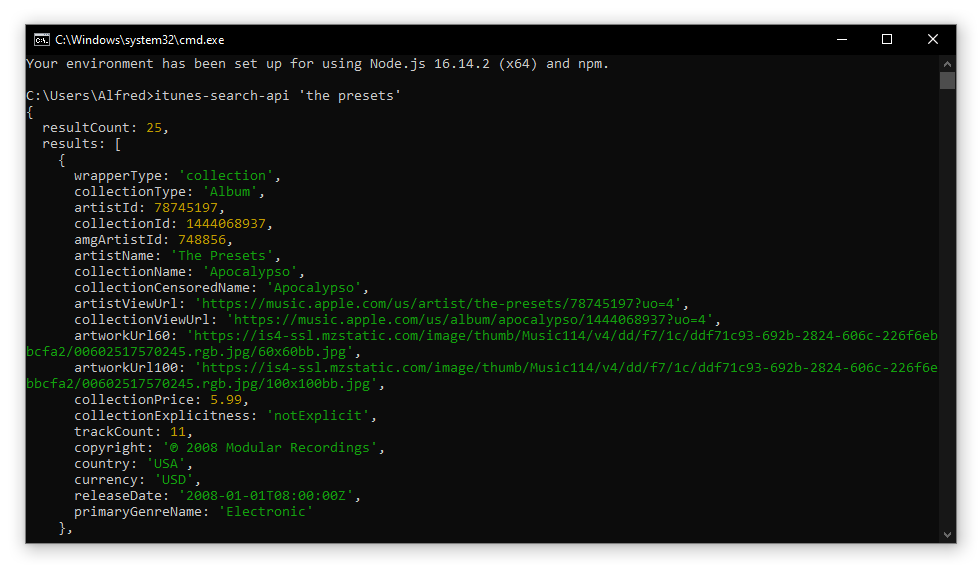
\includegraphics[width=0.75\linewidth]{itunesapi}
    \caption[Contoh penggunaan perkakas \itunesapi]{Contoh penggunaan perkakas \itunesapi. Gambar hanya memuat satu objek untuk menghemat tempat.}
    \label{fig:similarapps-itunesapi}
\end{figure}

\subsection{\ubercli\footnote{\href{https://github.com/jaebradley/uber-cli}{https://github.com/jaebradley/uber-cli}}}
\label{sec:similarapps-ubercli}

\ubercli merupakan sebuah perkakas \cl yang dapat digunakan untuk dua fungsi utama. Fungsi pertama dari perkakas ini adalah untuk mendapatkan estimasi untuk seberapa lama waktu yang diperlukan untuk servis taksi \textit{online} dari Uber untuk mencapai lokasi yang ingin dituju, sedangkan fungsi keduanya adalah untuk mengestimasi berapa harga yang harus dibayarkan untuk memakai servis tersebut. 
\newline\newline\noindent
Fungsi yang pertama dapat dilakukan memanggil perintah dengan format sebagai berikut.

\begin{verbatim}
                              uber time <alamat>
\end{verbatim}

\verb|uber| merupakan perintah dasar dari perkakas ini. \verb|time| merupakan parameter yang menandakan bahwa pengguna ingin menggunakan servis prediksi waktu dari perkakas ini. Selain itu, pengguna harus memasukkan alamat yang ingin dituju sebagai parameter akhir dari perintah yang akan digunakan sebagai masukan. Jika sintaksnya sudah benar, perintah tersebut akan bisa diproses oleh perkakas dengan cara mengirimkan pesan hasil konversi perintah tersebut ke API Uber. Setelah pemrosesan pesan tersebut berhasil, perkakas ini akan menampilkan sebuah keluaran dengan format yang dapat dilihat di gambar \ref{fig:similarapps-ubercli-time}. Perlu diperhatikan juga bahwa keluaran yang dihasilkan oleh perkakas ini akan meliputi seluruh jenis servis yang disediakan oleh Uber.

\begin{figure}[ht]
    \centering
    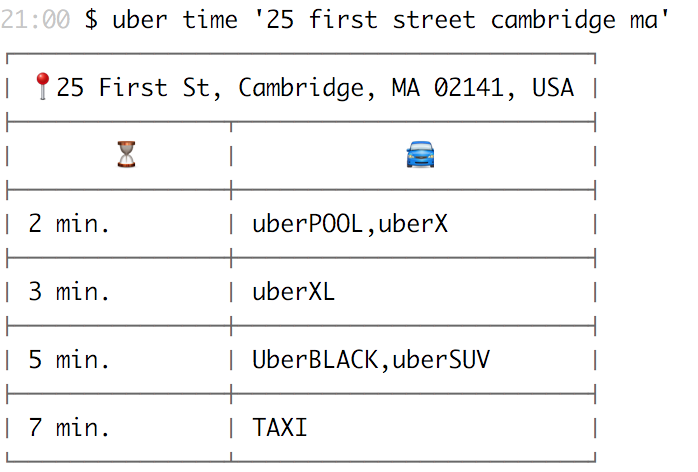
\includegraphics[width=0.425\linewidth]{ubercli-time}
    \caption[Contoh penggunaan perkakas \ubercli (\textit{time})]{Contoh penggunaan fitur prediksi waktu perjalanan untuk perkakas \ubercli.\protect\footnotemark}
    \label{fig:similarapps-ubercli-time}
\end{figure}
\footnotetext{\href{https://github.com/jaebradley/uber-cli}{https://github.com/jaebradley/uber-cli}}
\newpage\noindent % prevent code below from hanging off the very end of page
Sedangkan, untuk memanggil fungsi kedua dari perkakas ini, pengguna dapat dilakukan dengan memanggil perintah dengan format berikut.

\begin{verbatim}
                  uber price -s <alamat awal> -e <alamat akhir>
\end{verbatim}

Untuk sintaks ini, \verb|uber| memiliki fungsi yang sama dengan sintaks untuk fungsi pertama dari perkakas. \verb|price| merupakan penanda untuk perkakas bahwa pengguna ingin menggunakan servis untuk mengetahui perkiraan harga layanan Uber. Selanjutnya, perkakas akan meminta dua buah opsi beserta parameternya masing-masing. Pertama, opsi \verb|-s|, berarti \textit{start}, yang akan meminta sebuah parameter berupa lokasi yang ingin dipakai sebagai lokasi awal perkiraan harga layanan Uber. Sedangkan opsi \verb|-e|, berarti \textit{end}, akan meminta sebuah parameter berupa lokasi yang ingin dipakai sebagai lokasi akhir jasa perkiraan harga.
\newline\newline\noindent
Adapun keluaran dari fungsi kedua ini dapat dilihat di gambar \ref{fig:similarapps-ubercli-price}. Sama seperti keluaran untuk fungsi pertamanya, keluaran untuk fungsi kedua perkakas ini juga meliputi seluruh jasa yang disediakan oleh Uber.

\begin{figure}[ht]
    \centering
    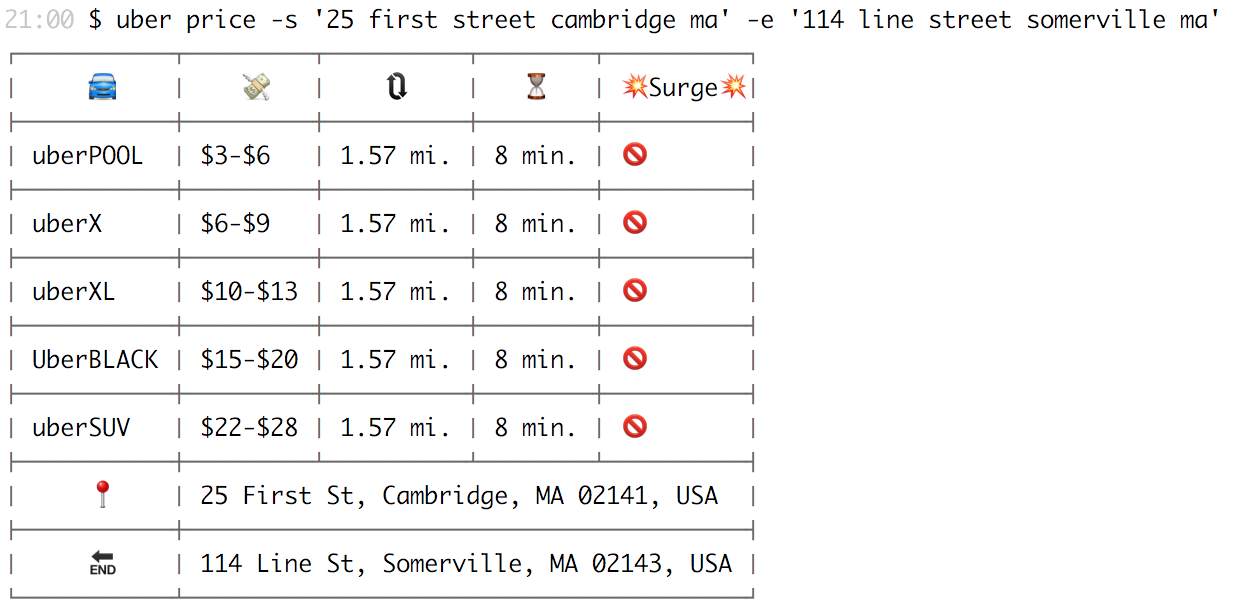
\includegraphics[width=0.75\linewidth]{ubercli-price}
    \caption[Contoh penggunaan perkakas \ubercli (\textit{price})]{Contoh penggunaan fitur prediksi harga perjalanan untuk perkakas \ubercli.\protect\footnotemark}
    \label{fig:similarapps-ubercli-price}
\end{figure}
\footnotetext{Gambar diambil dari \href{https://github.com/jaebradley/uber-cli}{https://github.com/jaebradley/uber-cli}}

\subsubsection{Permasalahan}
\label{sec:similarapps-ubercli-problem}

Seperti telah dijelaskan di awal bab ini, perkakas ini tidak dapat digunakan. Kesimpulan yang diambil oleh penulis mengenai alasan perkakas ini tidak dapat dijalankan adalah dikarenakan oleh penggunaan API dan modul-modul yang telah usang (\textit{deprecated}). Kesimpulan ini diambil oleh penulis karena dua alasan utama. Pertama, pada awalnya, perkakas ini tidak dapat dijalankan karena API Google \textit{Maps} yang dipakai mengandung baris kode berikut didalamnya.

\begin{verbatim}
           exports.placesAutoCompleteSessionToken = require('uuid/v4');
\end{verbatim}

Kode ini merupakan kode yang dipakai untuk mengambil \textit{subpath} dari paket \verb|uuid|, tetapi penggunaannya sudah berubah untuk versi yang lebih barunya. Akan tetapi, setelah diganti baris tersebut ke penggunaan versi barunya pun, perkakas ini masih tetap tidak dapat dijalankan\textemdash sekarang perkakas ini justru mengembalikan sebuah error. Singkatnya, error tersebut menunjukkan bahwa perkakas mencoba untuk mengakses API Uber dengan menggunakan kredensial OAuth 2.0 yang hanya berlaku untuk versi sebelumnya dari API tersebut. Permasalahan ini merupakan permasalahan yang juga ditemukan oleh beberapa pengguna lain, seperti tertera di halaman \textit{GitHub Issues} dari repositori ini.\footnote{\href{https://github.com/jaebradley/uber-cli/issues/87}{https://github.com/jaebradley/uber-cli/issues/87}} Oleh karena hal ini tidak lagi merupakan masalah kode perangkat lunak, maka perkakas ini dianggap tidak dapat dipakai.

\subsection{\googlemapscli\footnote{\href{https://github.com/yujinlim/google-maps-direction-cli}{https://github.com/yujinlim/google-maps-direction-cli}}}
\label{sec:similarapps-googlemapscli}

\googlemapscli merupakan sebuah perkakas \cl yang memiliki kegunaan yang mirip dengan KIRI, hanya saja perkakas ini tidak secara spesifik mengharuskan penggunaan angkot, atau transportasi umum lainnya. Singkatnya, perkakas ini memiliki fungsi seperti sebuah GPS. Untuk menggunakannya, pengguna harus memasukkan perintah dengan bentuk sebagai berikut.

\begin{verbatim}
                      direction <lokasi awal> <lokasi akhir>
\end{verbatim}

Setelah pengguna memasukkan perintah tersebut dengan benar, perkakas ini akan mengirim permintaan ke API Google \textit{Maps}, di mana jika prosesnya berhasil, keluarannya akan berupa langkah-langkah yang harus ditempuh untuk sampai ke lokasi akhir, beserta di jarak berapa langkah tersebut harus diambil, relatif terhadap langkah sebelumnya. Adapun penggunaan dari perkakas ini dapat dilihat di gambar \ref{fig:similarapps-googlemapscli}.

\begin{figure}[ht]
    \centering
    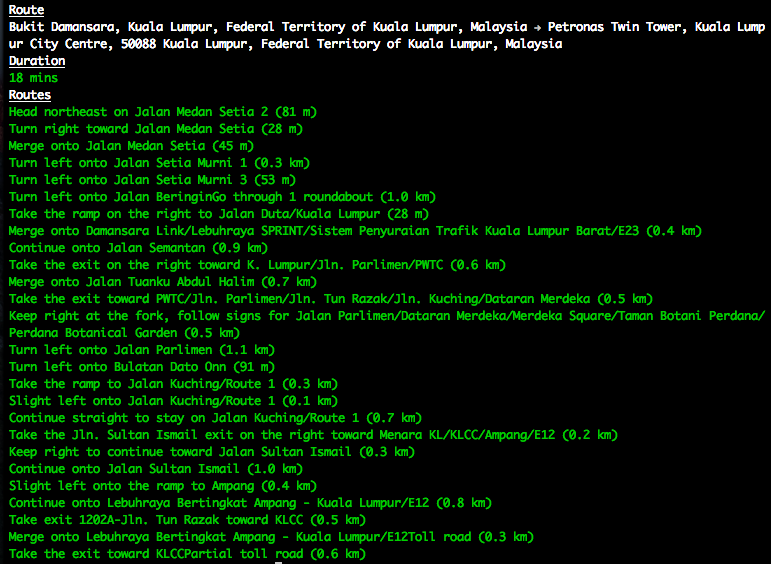
\includegraphics[width=0.66667\linewidth]{googlemapscli}
    \caption[Contoh penggunaan perkakas \googlemapscli]{Contoh penggunaan perkakas \googlemapscli.\protect\footnotemark}
    \label{fig:similarapps-googlemapscli}
\end{figure}
\footnotetext{Gambar diambil dari \href{https://github.com/yujinlim/google-maps-direction-cli}{https://github.com/yujinlim/google-maps-direction-cli}}

\subsubsection{Permasalahan}
\label{sec:similarapps-googlemapscli-problem}

Seperti tertulis di awal bab ini, perkakas ini juga tidak bisa digunakan. Alasan perkakas ini tidak dapat digunakan lagi-lagi merupakan masalah teknikal, yaitu diperbaruinya API Google \textit{Maps}. Lebih spesifiknya, semenjak 2018, \textit{Google} tidak lagi memperbolehkan penggunaan API Google \textit{Maps} tanpa kunci API, yang sayangnya tidak hanya mendasari perkakas ini, tetapi juga kunci API ini tidak bisa didapatkan tanpa membayarkan biaya tertentu. Oleh karena itu, perkakas ini dianggap tidak bisa lagi dijalankan.

\section{Analisis API KIRI}
\label{sec:analysis-kiri}

API KIRI memiliki tiga buah layanan, yaitu \textit{search place}, \textit{routing}, dan \textit{smart direction}. Di antara ketiga layanan ini, perlu diingat bahwa \textit{smart direction} merupakan sebuah layanan yang bekerja dengan langsung membuka halaman web KIRI sendiri, sehingga layanan ini tidak akan digunakan dalam pembuatan perkakas \cl untuk skripsi ini.

\subsection{\textit{Search Place}}
\label{sec:analysis-kiri-searchplace}

Layanan pertama dari dua layanan yang tersisa merupakan layanan \textit{search place.} Layanan ini merupakan layanan API KIRI yang berfungsi untuk mencari sebuah lokasi, beserta nilai \textit{latitude} dan \textit{longitude}-nya, berdasarkan kata kunci yang diberikan oleh pengguna. Untuk memanfaatkan layanan ini, sebuah permintaan GET harus dikirimkan ke alamat API KIRI. Adapun permintaan tersebut akan memiliki parameter-parameter sebagai berikut.

\begin{itemize}
	\item \verb|version|\\
	Parameter ini merupakan tanda bagi API untuk menggunakan protokol versi 2. Karena kemungkinan nilai untuk parameter ini hanya satu, maka parameter ini pasti bernilai \verb|2|.
	\item \verb|mode|\\
	Parameter ini merupakan mode dari servis/jasa API yang akan digunakan oleh pengguna. Untuk pengunaan layanan \textit{search place}, parameter ini diisi dengan \verb|searchplace|.
	\item \verb|region|\\
	Parameter ini mengatur daerah mana tempat lokasi yang ingin dicari berada. Isi dari parameter ini akan diberikan oleh pengguna pada saat pemakaian perkakas.
	\item \verb|querystring|\\
	Parameter ini akan berisi kata kunci yang diberikan oleh pengguna untuk mencari lokasi yang ingin ditemukan.
	\item \verb|apikey|\\
	Parameter ini akan berisi sebuah nilai kunci API yang sudah dibuat sebelumnya, seperti dijelaskan di subbab \ref{sec:kiri-api}, parameter ini akan bernilai \verb|68C|\apikeycensor \verb|97C|.\footnote{Kunci API ditutupi untuk alasan keamanan.}
\end{itemize}

\subsection{\textit{Routing}}
\label{sec:analysis-kiri-findroute}

Layanan kedua dari API ini merupakan fungsi utama dari KIRI sendiri, yaitu pencarian rute dengan menggunakan angkot. Layanan ini akan menerima dua buah lokasi yang ingin dijadikan lokasi awal dan lokasi akhir, dan menunjukkan langkah-langkah yang harus ditempuh untuk menempuh perjalanan tersebut, dengan memanfaatkan jasa angkot yang ada. Sama seperti layanan \textit{search place}, layanan ini juga digunakan dengan mengirimkan permintaan GET ke alamat API KIRI.

\begin{itemize}
	\item \verb|version|\\
	Sama seperti pada layanan \textit{search place}, parameter ini hanya dapat diisi dengan nilai \verb|2|.
	\item \verb|mode|\\
	Parameter ini merupakan mode dari servis/jasa API yang akan digunakan oleh pengguna. Untuk pengunaan layanan \textit{routing}, parameter ini diisi dengan \verb|findroute|.
	\item \verb|locale|\\
	Isi dari parameter ini akan ditentukan pada saat pemakaian perkakas.
	\item \verb|start|\\
	Parameter ini merupakan nilai \latlon dari titik awal perjalanan pengguna, yang akan diberikan sebagai masukan pada saat pemakaian perkakas.
	\item \verb|finish|\\
	Parameter ini merupakan nilai \latlon dari titik akhir/tujuan perjalanan pengguna, yang akan diberikan sebagai masukan pada saat pemakaian perkakas.
	\item \verb|presentation|\\
	Parameter ini hanya digunakan untuk fitur \textit{backwards compatibility}. Jika parameter ini ingin digunakan, maka isi dari parameter ini hanya ada satu kemungkinan, yaitu \verb|desktop|. Jika parameter ini tidak dipakai
	\item \verb|apikey|\\
	Sama seperti pada layanan \textit{search place}, parameter ini akan berisi sebuah nilai kunci API yang sudah dibuat sebelumnya, yaitu \verb|68C|\apikeycensor \verb|97C|.
\end{itemize}
\vspace{\baselineskip}\noindent
Layanan ini dapat digunakan sebagai lanjutan dari layanan \textit{search place}, terutama karena fitur pencarian rute hanya menerima nilai \latlon dari lokasi-lokasi yang akan digunakan sebagai masukan, yang tidak hanya akan menyusahkan pengguna dalam memakai perkakas \cl ini, tetapi juga kedua nilai tersebut juga merupakan salah satu dari keluaran layanan pencarian lokasi. Jadi, dengan menggunakan kedua layanan tersebut secara berlangsungan, maka pengguna hanya perlu mencari lokasi tersebut dengan kata-kata kunci, dan pada akhirnya pengguna akan dapat menerima langkah-langkah yang harus ditempuh dalam rute sebagai keluaran akhir dari perkakas.

\section{Analisis Perkakas yang Akan Dibuat}
\label{sec:analysis-thesisapp}

Di bagian ini akan dibahas analisis hal-hal yang berhubungan dengan perkakas yang akan dibangun sebagai proyek skripsi ini.

\subsection{Analisis Fitur Perkakas}
\label{sec:analysis-thesisapp-functions}

Pada skripsi ini, akan dibangun sebuah aplikasi berupa perkakas \cl yang merupakan ekstensi dari sebuah aplikasi berbasis web lain, yaitu KIRI. Perkakas ini akan menjadi ekstensi KIRI dengan cara memungkinkan penggunanya untuk mengakses fungsi-fungsi API KIRI dari \cl milik perangkat mereka masing-masing. Fungsi utama dari perkakas ini tentunya sama dengan KIRI sendiri, yaitu membantu navigasi dari satu lokasi ke lokasi lain dengan menggunakan angkot.

Walaupun begitu, aplikasi ini akan memiliki dua fungsi utama yang berhubungan satu sama lain, yaitu pencarian lokasi, dan penunjukkan rute dengan angkot.

\begin{itemize}
	\item Pencarian lokasi\\
	Pencarian lokasi merupakan fungsi utama pertama dari perkakas ini. Untuk fungsi ini, masukan langsung dari pengguna yang akan diterima oleh perkakas adalah kata kunci dari sebuah lokasi yang ingin dicari. Kemudian, perkakas akan memprosesnya melalui API KIRI, lalu mengembalikan nama lokasi tersebut, serta nilai \textit{latitude} dan \textit{longitude}-nya, sebagai keluaran akhir dari proses tersebut.
	\item Pencarian rute\\
	Pencarian rute dengan angkot merupakan fungsi utama kedua, sekaligus fungsi umum dari perkakas ini. Dalam fungsi ini, perkakas akan meminta masukan langsung pengguna berupa nilai \latlon dari lokasi awal serta lokasi akhir dari perjalanan pengguna. Setelah masukan ini berhasil diterima dan diproses, perkakas akan mengeluarkan keluaran akhir berupa langkah-langkah yang harus diambil oleh pengguna untuk pergi dari lokasi awal ke lokasi akhir, dengan memanfaatkan jasa angkot yang ada.
\end{itemize}
\vspace{\baselineskip}\noindent
Berikut merupakan opsi-opsi yang akan disediakan dalam perkakas yang akan dibangun.

\begin{itemize}
	\item \verb|-h|\\
	Perlu diingat juga bahwa aplikasi ini merupakan aplikasi \cl murni, yang berarti bahwa seluruh operasi dari aplikasi ini akan dilakukan tanpa bantuan gambar grafis apapun. Untuk membantu penggunanya dalam mengetahui bagaimana cara menggunakan perkakas ini, tentunya perintah untuk menunjukkan apa perintah-perintah dan opsi-opsi yang tersedia merupakan sebuah keharusan. Hal ini merupakan fungsi satu-satunya dari perintah \verb|--help| ini.
	
	\item \verb|-m <mode>|\\
	Opsi ini merupakan opsi berparameter yang menentukan fitur mana yang ingin digunakan oleh pengguna. Adapun isi dari parameter \verb|mode| yang dapat digunakan adalah sebagai berikut:
	
	\begin{itemize}	
		\item \verb|search|\\
		Parameter ini akan menandakan bahwa pengguna ingin menggunakan fitur \textit{search place} dari perkakas. Untuk mode ini, perkakas akan menerima input dari pengguna dalam bentuk parameter-parameter dari opsi-opsi tambahan. Adapun opsi-opsi tersebut adalah sebagai berikut.
			
		\begin{itemize}
			\item \verb|-r <region>|\\
			Opsi ini merupakan opsi yang akan menerima parameter berupa kode area dari lokasi yang ingin dicari.
			\item \verb|-q <kata kunci>|\\
			Opsi ini merupakan opsi yang akan menerima sebuah \textit{string} sebagai parameternya. \textit{String} ini akan digunakan oleh perkakas sebagai kata kunci untuk pencarian lokasi yang ingin ditemukan oleh pengguna.
		\end{itemize}
	
		\item \verb|route|\\
		Parameter ini akan menandakan bahwa pengguna ingin menggunakan fitur \textit{find route} dari perkakas. Sama seperti mode \verb|--search|, perkakas akan menerima input dari pengguna dari parameter-parameter milik opsi-opsi tambahan. Adapun opsi-opsi tersebut adalah sebagai berikut.
		
		\begin{itemize}
			\item \verb|-s <lokasi awal>|\\
			Opsi ini merupakan opsi yang akan menerima parameter berupa lokasi awal perjalanan pengguna nantinya. Perlu diingat bahwa opsi ini hanya menerima masukan lokasi berupa nilai \latlon dari lokasi tersebut.
			\item \verb|-f <lokasi akhir>|\\
			Opsi ini merupakan opsi yang akan menerima parameter berupa lokasi akhir perjalanan pengguna nantinya. Sama seperti opsi sebelumnya, parameter ini juga hanya menerima masukan lokasi berupa nilai \textit{latitude} dan \textit{longitude}.
			\item \verb|-l <kode bahasa>|\\
			Opsi ini akan menerima parameter yang mengatur bahasa yang akan digunakan oleh perkakas di keluarannya nanti.
		\end{itemize}
		
		\item \verb|routedirect|\\
		Parameter ini merupakan tambahan fitur spesifik untuk perkakas ini, yang merupakan gabungan dari fitur pencarian lokasi dan pencarian rute. Fitur ini akan menggabungkan kedua fitur tersebut dengan langkah-langkah berikut.
		
		\begin{enumerate}
			\item Perkakas akan menerima lokasi awal dan akhir berupa kata kunci dari pengguna yang dimasukkan kedalam parameter dari opsi masing-masing.
			\item Hasil pencarian kedua lokasi akan dikonfirmasi terlebih dahulu, apakah lokasi yang ditemukan benar merupakan lokasi yang ingin digunakan oleh pengguna atau bukan.
			\item Jika hasil tersebut benar, maka koordinat \latlon dari kedua lokasi tersebut akan disimpan.
			\item Koordinat \latlon dari kedua lokasi tersebut kemudian akan digunakan sebagai masukan untuk langkah kedua dari fitur ini, yaitu pencarian rute.
			\item Hasil dari pencarian rute akan ditampilkan sebagai keluaran akhir dari fitur ini.
		\end{enumerate}
		\noindent
		Adapun parameter yang diperlukan untuk fitur ini merupakan gabungan dari opsi-opsi kedua fitur sebelumnya, yaitu:
		
		\begin{itemize}
			\item \verb|-I <region tempat lokasi awal berada>|\\
			Opsi ini akan menerima parameter berupa kode area dari lokasi awal yang akan digunakan.
			\item \verb|-E <region tempat lokasi akhir berada>|\\
			Opsi ini akan menerima parameter berupa kode area dari lokasi akhir yang akan digunakan.
			\item \verb|-S <kata kunci untuk lokasi awal>|\\
			Opsi ini akan menerima parameter berupa kata kunci untuk pencarian lokasi awal yang akan digunakan.
			\item \verb|-F <kata kunci untuk lokasi akhir>|\\
			Opsi ini akan menerima parameter berupa kata kunci untuk pencarian lokasi akhir yang akan digunakan.
			\item \verb|-l <kode bahasa>|\\
			Opsi ini akan menerima parameter yang mengatur bahasa yang akan digunakan oleh perkakas di keluarannya nanti. Opsi ini merupakan opsi yang sama dengan opsi yang digunakan dalam mode \verb|route|.
		\end{itemize}
		
	\end{itemize}
	
\end{itemize}

\subsection{Analisis \textit{Use Case}}
\label{sec:analysis-thesisapp-usecases}

Perkakas \cl ini akan memiliki dua fitur, yaitu pencarian lokasi dan pencarian rute dengan angkot. Oleh karena itu, diagram \textit{use case} dari aplikasi ini akan mengandung dua \textit{use case}, yang dapat dilihat di gambar \ref{fig:thesisapp-uml}. Adapun penjelasan dari tiap-tiap \textit{use case} tersebut dapat dilihat di tabel \ref{tab:thesisapp-scenariocase-searchplace}, tabel \ref{tab:thesisapp-scenariocase-findroute}, dan tabel \ref{tab:thesisapp-scenariocase-findroutedirect}.

\begin{figure}[ht]
    \centering
    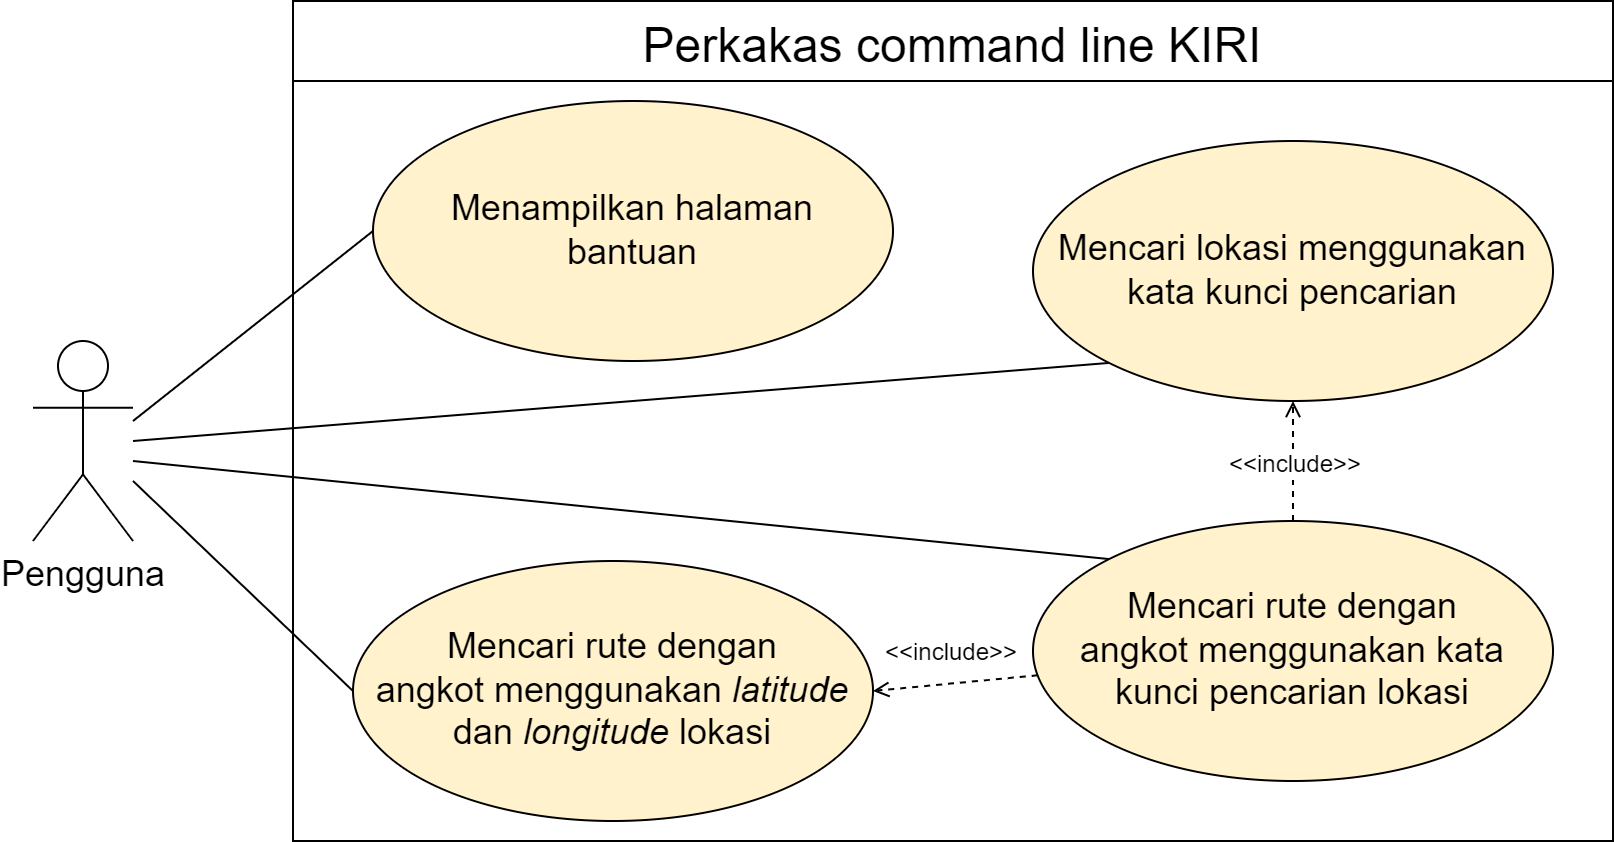
\includegraphics[width=0.5\linewidth]{thesisapp-uml}
    \caption[Diagram \textit{use case} perkakas yang akan dibangun]{Diagram \textit{use case} dari perkakas yang akan dibangun.}
    \label{fig:thesisapp-uml}
\end{figure}

\begin{table}[H]
    \centering
    \begin{tabular}{|p{3cm}|p{10cm}|}
    \hline
        Nama & Mencari lokasi\\
    \hline
    \hline
        Deskripsi & Fitur untuk mencari lokasi di area tertentu berdasarkan kata kunci\\
    \hline
		Aktor & Pengguna aplikasi\\
	\hline
		Pre-kondisi & -\\
    \hline
		Pos-kondisi & Nama dari lokasi serta koordinat \textit{latitude} dan \textit{longitude}-nya ditampilkan kepada pengguna.\\
    \hline
		Skenario utama & 
		\begin{enumerate}
			\item Perkakas membaca masukan dari argumen dalam perintah \cl.
			\item Perkakas memproses masukan tersebut dan mengirimkannya ke API KIRI untuk diproses lebih lanjut.
			\item Perkakas menerima keluaran dari API KIRI dan  meneruskannya kembali kepada pengguna.
        \end{enumerate}\\
    \hline
		Skenario eksepsi & Pengguna memasukkan masukan yang tidak valid di dalam salah satu parameter.\\
	\hline
    \end{tabular}
    \caption{\textit{Scenario case} untuk fitur pencarian rute dengan angkot.}
    \label{tab:thesisapp-scenariocase-searchplace}
\end{table}

\begin{table}[H]
    \centering
    \begin{tabular}{|p{3cm}|p{10cm}|}
    \hline
        Nama & Mencari rute dengan angkot menggunakan \latlon lokasi\\
    \hline
    \hline
        Deskripsi & Fitur untuk mencari cara pergi ke satu lokasi ke lokasi lainnya dengan menggunakan angkot dengan nilai \latlon lokasi sebagai masukan.\\
    \hline
		Aktor & Pengguna aplikasi\\
	\hline
		Pre-kondisi & Pengguna menyiapkan lokasi awal dan lokasi akhir berupa koordinat \textit{latitude} dan \textit{longitude}.\\
    \hline
		Pos-kondisi & Langkah-langkah yang harus ditempuh untuk perjalanan tersebut akan ditampilkan kepada pengguna.\\
    \hline
		Skenario utama & 
		\begin{enumerate}
			\item Perkakas membaca masukan dari argumen dalam perintah \cl, berupa nilai \latlon dari lokasi.
			\item Perkakas memproses masukan tersebut dan mengirimkannya ke API KIRI untuk diproses lebih lanjut.
			\item Perkakas menerima keluaran dari API KIRI dan meneruskannya kembali kepada pengguna.
        \end{enumerate}\\
	\hline
		Skenario eksepsi & Pengguna memasukkan masukan yang tidak valid di dalam salah satu parameter.\\
    \hline
    \end{tabular}
    \caption{\textit{Scenario case} untuk fitur pencarian rute dengan angkot, dengan nilai \latlon kedua lokasi sebagai masukan.}
    \label{tab:thesisapp-scenariocase-findroute}
\end{table}

\begin{table}[H]
    \centering
    \begin{tabular}{|p{3cm}|p{10cm}|}
    \hline
        Nama & Mencari rute dengan angkot menggunakan kata kunci lokasi\\
    \hline
    \hline
        Deskripsi & Fitur untuk mencari cara pergi ke satu lokasi ke lokasi lainnya dengan menggunakan angkot dengan nilai \latlon lokasi sebagai masukan.\\
    \hline
		Aktor & Pengguna aplikasi\\
	\hline
		Pre-kondisi & -\\
    \hline
		Pos-kondisi & Langkah-langkah yang harus ditempuh untuk perjalanan tersebut akan ditampilkan kepada pengguna.\\
    \hline
		Skenario utama & 
		\begin{enumerate}
			\item Perkakas membaca masukan dari argumen dalam perintah \cl, berupa kata kunci pencarian lokasi.
			\item Perkakas memproses masukan tersebut dan mengirimkannya ke API KIRI untuk diproses lebih lanjut.
			\item Perkakas menerima keluaran dari API KIRI berupa hasil pencarian lokasi dan meneruskannya kembali ke pengguna untuk dikonfirmasi kebenarannya.
			\item Jika lokasi-lokasi tersebut...
			
			\begin{itemize}
				\item ...benar, maka perkakas akan meneruskan nilai \latlon yang didapatkan ke API KIRI lagi untuk diproses lebih lanjut.
				\item ...salah, maka proses akan diulangi dari langkah 1.
			\end{itemize}						
			
			\item Perkakas menerima keluaran akhir dari API KIRI berupa langkah-langkah dalam rute yang perlu ditempuh.
        \end{enumerate}\\
	\hline
		Skenario eksepsi & 
		\begin{itemize}
			\item Pengguna memasukkan masukan yang tidak valid di dalam salah satu parameter.
			\item Lokasi yang dicari dalam langkah 2 tidak ditemukan.
		\end{itemize}\\
    \hline
    \end{tabular}
    \caption{\textit{Scenario case} untuk fitur pencarian rute dengan angkot, dengan kata kunci kedua lokasi sebagai masukan.}
    \label{tab:thesisapp-scenariocase-findroutedirect}
\end{table}
